% Reset dei contatori per l'appendice
\setcounter{figure}{0}
\renewcommand{\thefigure}{A.\arabic{figure}}
\setcounter{table}{0}
\renewcommand{\thetable}{A.\arabic{table}}

\section{Analisi Approfondita degli Errori e Calibrazione}
\label{app:error_analysis}

Al fine di validare l'idoneità del modello \textit{Champion} (XGBoost Tuned) per l'impiego in ambiente produttivo, è stata condotta un'analisi diagnostica estesa. Tale indagine si è focalizzata su tre dimensioni critiche: la struttura della matrice di confusione, il potere discriminante (Ranking Ability) e l'affidabilità delle probabilità predette (Reliability).

\subsection{Analisi degli Errori di Classificazione}

La scomposizione delle predizioni attraverso le Matrici di Confusione (Figura \ref{fig:matrice_confusione.png}) permette di valutare il trade-off operativo tra precisione e copertura.

\begin{figure}[H]
    \centering
    % Placeholder per l'immagine Plotly (Matrici di Confusione)
    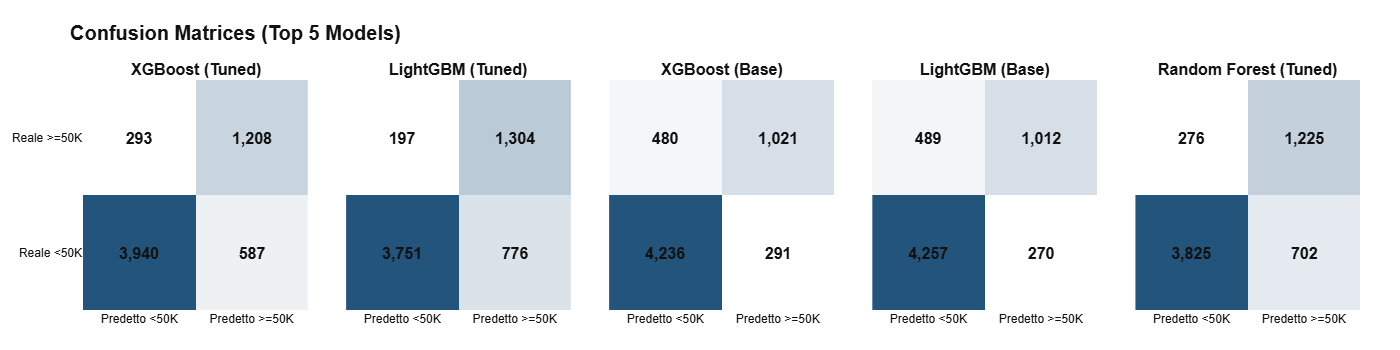
\includegraphics[width=\textwidth]{figures/matrice_confusione.png} 
    \caption{Confronto delle matrici di confusione per i modelli Top-5. Le celle diagonali (bianco e rosso scuro) rappresentano le classificazioni corrette.}
    \label{fig:matrice_confusione.png}
\end{figure}

\noindent
Il modello XGBoost Tuned mostra una robusta gestione della classe maggioritaria ($\le 50K$), minimizzando i Falsi Positivi. Tuttavia, si osserva un tasso fisiologico di Falsi Negativi (individui ad alto reddito classificati erroneamente come basso reddito), attribuibile alla sovrapposizione distributiva delle feature socio-demografiche nelle zone di confine decisionale.

\subsection{Metriche di Ranking (ROC e Precision-Recall)}

Poiché l'output primario del modello è uno score probabilistico $P(y=1|x)$, è fondamentale valutare la sua capacità di ordinare correttamente i casi positivi rispetto ai negativi, indipendentemente dalla soglia di classificazione.

\subsection{Curva ROC e AUC}
Tutti i modelli basati su Gradient Boosting mostrano prestazioni eccellenti, con un'Area Under Curve (AUC) superiore a $0.93$ (Tabella \ref{tab:auc_ranking}).
\begin{table}[H]
\centering
\begin{tabular}{lcc}
\toprule
\textbf{Modello} & \textbf{AUC-ROC} & \textbf{Rank} \\
\midrule
LightGBM (Tuned) & 0.9322 & 1 \\
XGBoost (Base) & 0.9319 & 2 \\
LightGBM (Base) & 0.9312 & 3 \\
\bottomrule
\end{tabular}
\caption{Ranking basato su AUC. Le differenze tra i primi tre modelli sono marginali ($<0.001$), indicando una sostanziale equivalenza nel potere discriminante.}
\label{tab:auc_ranking}
\end{table}


\begin{figure}[H]
    \centering
    % Placeholder per l'immagine Plotly (Matrici di Confusione)
    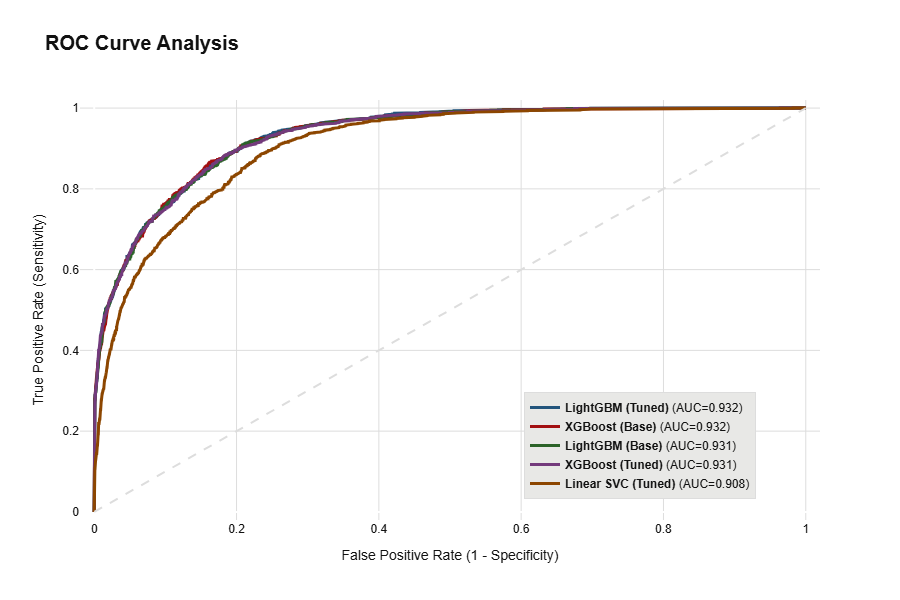
\includegraphics[width=\textwidth]{figures/roc.png} 
    \caption{AUC-ROC dei 5 modelli più performati con LightGBM (Tuned) e XGBoost (Base) valutaticome i migliori}
    \label{fig:roc.png}
\end{figure}

\subsection{Precision-Recall (PR) Curve}
In contesti sbilanciati, l'Average Precision (AP) è una metrica più informativa dell'AUC. LightGBM (Tuned) domina questa classifica con un AP di \textbf{0.8427}, dimostrando una superiorità nel mantenere alta la precisione anche a livelli elevati di recall, una caratteristica cruciale per minimizzare i falsi allarmi.


\begin{figure}[H]
    \centering
    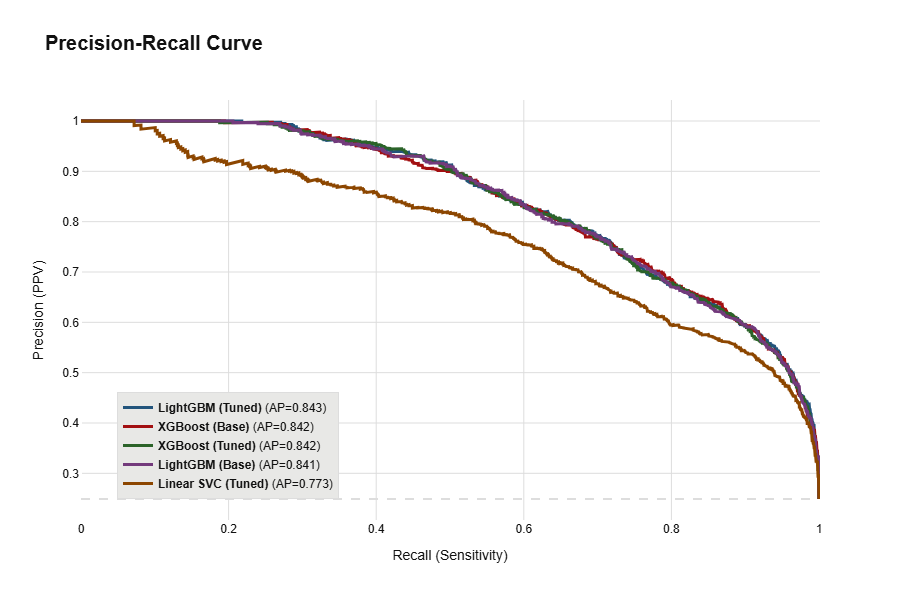
\includegraphics[width=\textwidth]{figures/prc.png} 
    \caption{Il confronto tra i modelli mostra prestazioni molto simili per LightGBM e XGBoost ($AP \approx 0.84$), che mantengono valori di precision elevati lungo gran parte del range di recall. Il Linear SVC presenta invece performance inferiori (AP = 0.773), con una diminuzione più marcata della precision all’aumentare della recall.}
    \label{fig:prc.png}
\end{figure}

\subsection{Analisi di Calibrazione (Reliability)}

Un modello è "ben calibrato" se la probabilità predetta riflette la frequenza empirica dell'evento (e.g., tra tutti i casi predetti con probabilità 0.7, il 70\% dovrebbe essere effettivamente positivo).
L'analisi mediante \textit{Calibration Plot} e \textbf{Brier Score} (Tabella \ref{tab:calibration}) conferma l'eccellenza di LightGBM.

\begin{table}[h]
\centering
\begin{tabular}{lcc}
\toprule
\textbf{Modello} & \textbf{Brier Score} (Lower is better) & \textbf{Rank} \\
\midrule
\textbf{LightGBM (Tuned)} & \textbf{0.0876} & \textbf{1} \\
CatBoost (Tuned) & 0.0878 & 2 \\
XGBoost (Tuned) & 0.0880 & 3 \\
\bottomrule
\end{tabular}
\caption{Valutazione della calibrazione probabilistica. LighXGBoost (Base) ottiene il punteggio Brier più basso, indicando stime di probabilità altamente affidabili.}
\label{tab:calibration}
\end{table}

\noindent
Il basso Brier Score (0.0876) indica che XGBoost (Base) produce probabilità predittive complessivamente accurate e ben calibrate. Pertanto, le stime possono essere utilizzate per decisioni di business (es. risk scoring), pur potendo valutare eventuali tecniche di ricalibrazione per ulteriori miglioramenti.

\subsection{Comparazione Grafica della Calibrazione}

A completamento della validazione statistica, il modello \textit{Champion} e i principali competitor sono stati sottoposti a una diagnostica strutturale volta a valutarne l'efficienza computazionale, i driver decisionali e la stabilità rispetto al rischio di overfitting.

\begin{figure}[H]
    \centering
    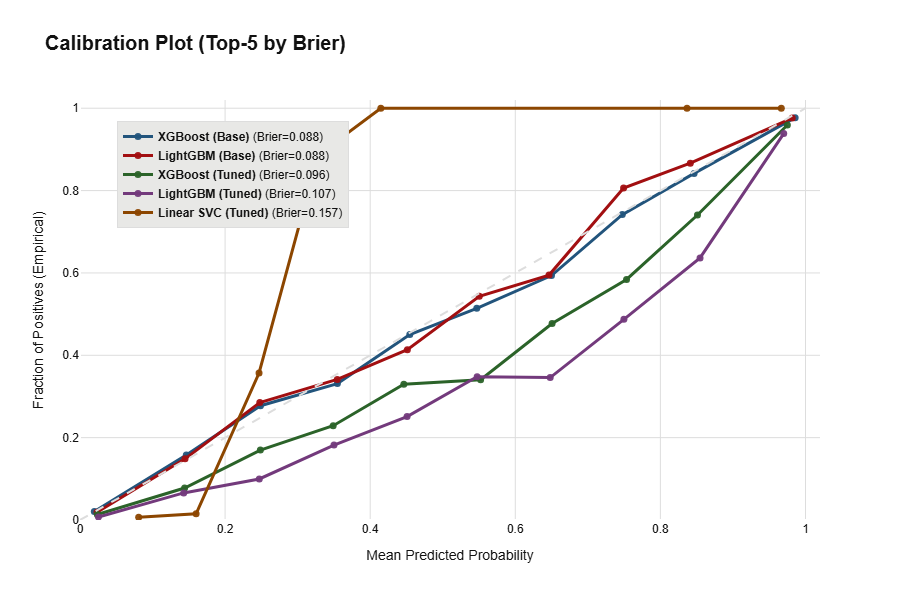
\includegraphics[width=\textwidth]{figures/calibration.png} 
    \caption{I modelli XGBoost e LightGBM nella versione base mostrano la calibrazione migliore ($Brier \approx 0.088$), con curve vicine alla diagonale ideale. Le versioni tuned presentano una calibrazione leggermente peggiore, mentre Linear SVC evidenzia la performance più bassa ($Brier \approx 0.157$).}
    \label{fig:calibration.png}
\end{figure}

\subsection{Frontiera di Efficienza (Time-Accuracy Trade-off)}

L'analisi comparativa dei costi computazionali (Tabella \ref{tab:efficiency}) evidenzia differenti profili di utilizzo risorse.
Sebbene \textbf{Linear SVC (Tuned)} risulti l'algoritmo più rapido in fase di inferenza (\(t_{inf} \approx 67\)ms), il modello selezionato \textbf{XGBoost (Tuned)} offre un compromesso globale accettabile, garantendo il massimo F1-Score (0.7330) con un tempo di latenza ampiamente contenuto (\(t_{inf} \approx 114\)ms), pienamente compatibile con requisiti di batch scoring o real-time moderato.

\begin{table}[H]
\centering
\begin{tabular}{lcc}
\toprule
\textbf{Modello} & \textbf{Latenza Inferenza (s)} & \textbf{F1-Score} \\
\midrule
Linear SVC (Tuned) & 0.0667 & 0.6840 \\
LightGBM (Base) & 0.0914 & 0.7273 \\
XGBoost (Base) & 0.1121 & 0.7259 \\
\textbf{XGBoost (Tuned)} & \textbf{0.1135} & \textbf{0.7330} \\
LightGBM (Tuned) & 0.2313 & 0.7283 \\
\bottomrule
\end{tabular}
\caption{Analisi trade-off efficienza/efficacia. le performances predittive con un overhead computazionale accettabile.}
\label{tab:efficiency}
\end{table}

\begin{figure}[H]
    \centering
    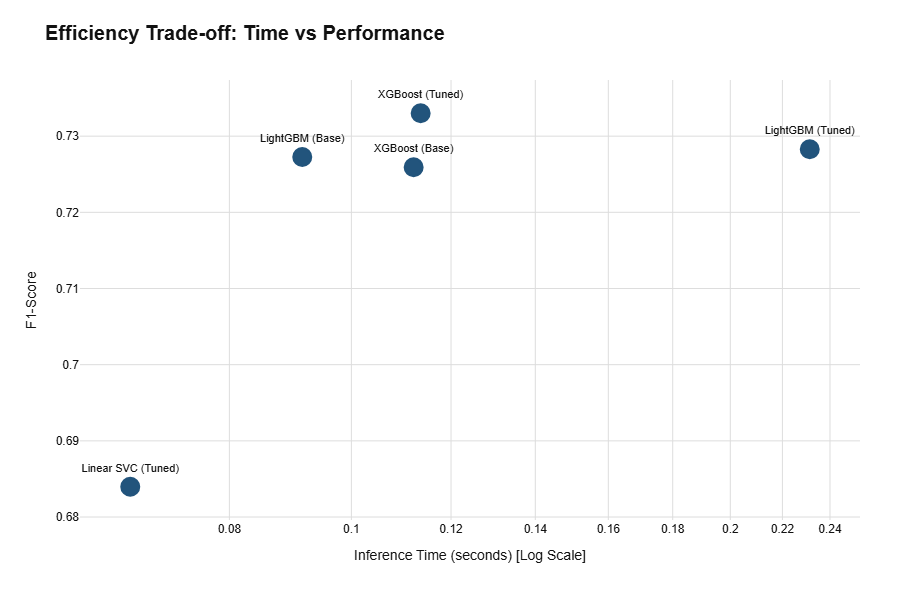
\includegraphics[width=\textwidth]{figures/time.png} 
    \caption{Il grafico mostra comem si distribuiscono i modelli nella loro performance di addestramento in relazione al tempoimpiegato.}
    \label{fig:time.png}
\end{figure}


\subsection{Feature Importance e Interpretabilità Globale}

Per comprendere i driver latenti del processo decisionale, è stata estratta la classifica delle feature. L'analisi per il modello vincitore \textbf{XGBoost (Tuned)} (Figura \ref{fig:FI_X.png}) si basa sull'importanza calcolata tramite il parametro \textit{Gain} (la riduzione dell'impurità media apportata da ciascuna variabile) e rivela una struttura gerarchica molto chiara:

\begin{enumerate}
    \item \textbf{Dominanza dello Stato Civile e Relazioni:} La variabile dummy \texttt{marital.status\_Married-civ-spouse} risulta di gran lunga il discriminante principale (con un Gain di circa 0.32), seguita da altre variabili relazionali come \texttt{relationship\_Husband}. Questo indica che la stabilità familiare e la probabilità di un doppio reddito aggregato costituiscono il fattore più predittivo per il superamento della soglia dei 50K.
    \item \textbf{Capitale Finanziario:} \texttt{capital.gain} emerge come il secondo driver più forte in assoluto, confermando che l'accumulazione di ricchezza tramite investimenti finanziari diretti è un indicatore inequivocabile di reddito elevato.
    \item \textbf{Istruzione e Professione:} \texttt{education.num} mantiene un peso cruciale nel modello, supportando la teoria del capitale economico legato alle competenze. Parallelamente emergono categorie professionali ad alto reddito come \texttt{occupation\_Exec-managerial}.
\end{enumerate}

\noindent
Al contrario, osservando le metriche estratte da \textbf{LightGBM} (Figura \ref{fig:FI_L.png}), si nota una predilezione netta per le variabili continue (\texttt{age}, \texttt{hours.per.week}). Questo comportamento è tipico quando l'importanza viene misurata in base alla metrica di \textit{Split} (frequenza di taglio nei rami dell'albero), che tende fisiologicamente a premiare le variabili ad alta cardinalità rispetto alle categoriche, offrendo molteplici punti di segmentazione. Entrambe le gerarchie, seppur calcolate in modo diverso, validano la plausibilità semantica e le aspettative di dominio economico dell'esperimento.

\begin{figure}[H]
    \centering
    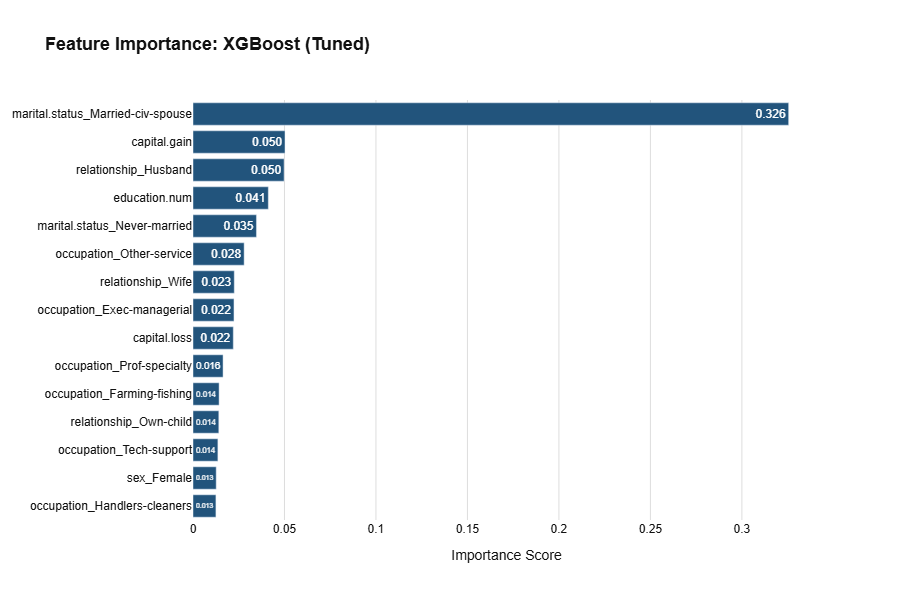
\includegraphics[width=\textwidth]{figures/FI_X.png} 
    \caption{Importanza delle feature per il modello XGBoost (Tuned), misurata tramite Gain. Lo stato civile domina nettamente la capacità predittiva.}
    \label{fig:FI_X.png}
\end{figure}

\begin{figure}[H]
    \centering
    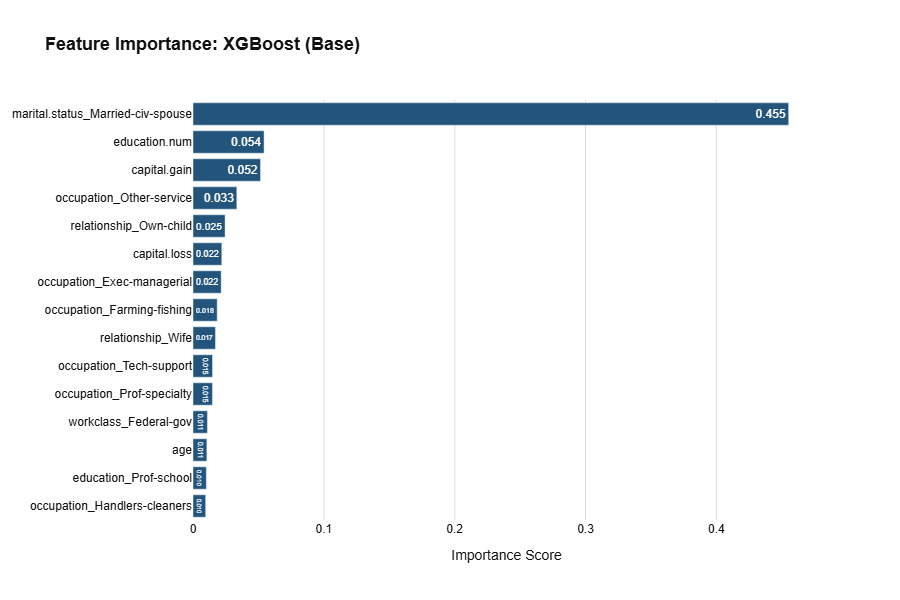
\includegraphics[width=\textwidth]{figures/FI_XB.png} 
    \caption{Importanza delle feature per il modello XGBoost (Base).}
    \label{fig:FI_XB.png}
\end{figure}

\begin{figure}[H]
    \centering
    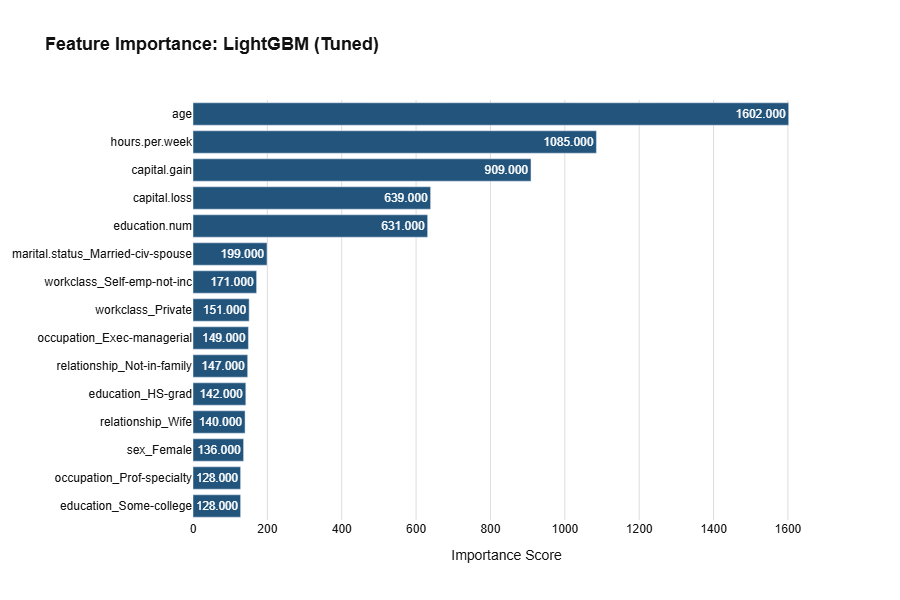
\includegraphics[width=\textwidth]{figures/FI_L.png} 
    \caption{Importanza delle feature per il modello LightGBM (Tuned). A differenza di XGBoost, le variabili continue dominano la classifica a causa dell'impatto della metrica di conteggio degli split.}
    \label{fig:FI_L.png}
\end{figure}

\begin{figure}[H]
    \centering
    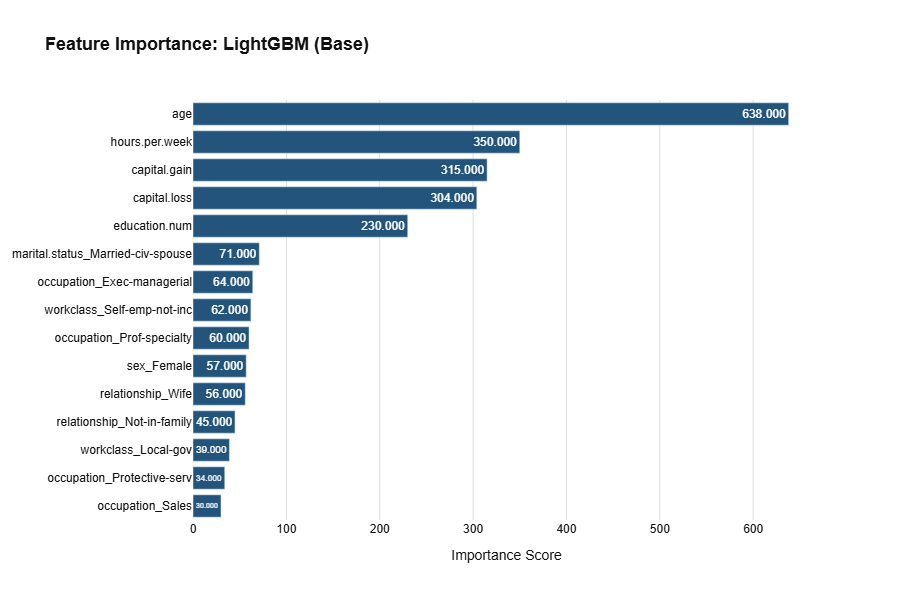
\includegraphics[width=\textwidth]{figures/FI_LB.png} 
    \caption{Importanza delle feature per il modello LightGBM (Base).}
    \label{fig:FI_LB.png}
\end{figure}


\section{Analisi del Rischio di Overfitting (Generalization Gap)}

La stabilità della generalizzazione è stata quantificata misurando il \textit{Gap} tra l'accuratezza sul set di training (\(Acc_{train}\)) e quella sul set di test (\(Acc_{test}\)). Un gap ridotto è indice di un modello che apprende pattern robusti senza memorizzare il rumore statistico del campione di addestramento.

\begin{table}[h]
\centering
\begin{tabular}{lccc}
\toprule
\textbf{Modello} & \textbf{Acc. Train} & \textbf{Acc. Test} & \textbf{Gap (\(\Delta\))} \\
\midrule
Linear SVC (Tuned) & 0.8026 & 0.8021 & 0.0005 \\
LightGBM (Base) & 0.8832 & 0.8741 & 0.0091 \\
LightGBM (Tuned) & 0.8565 & 0.8386 & 0.0179 \\
XGBoost (Base) & 0.8924 & 0.8721 & 0.0203 \\
\textbf{XGBoost (Tuned)} & \textbf{0.8779} & \textbf{0.8540} & \textbf{0.0239} \\
\bottomrule
\end{tabular}
\caption{Analisi del Generalization Gap. Tutti i modelli mostrano un rischio di overfitting "Basso" (\(\Delta \le 0.05\)).}
\label{tab:overfitting_gap}
\end{table}

\noindent
I risultati (Tabella \ref{tab:overfitting_gap}) dimostrano l'efficacia delle tecniche di regolarizzazione impiegate. Modelli lineari più semplici come la \textbf{Linear SVC} presentano fisiologicamente un gap pressoché nullo (\(0.05\%\)), a fronte però di un potere predittivo inferiore. Il modello vincitore \textbf{XGBoost (Tuned)} mantiene un gap decisamente contenuto (\(\approx 2.4\%\)), significativamente inferiore alla soglia di attenzione del 5\%. Questo garantisce che le prestazioni osservate in fase di test siano una stima affidabile e solida del comportamento futuro del modello in un ambiente di produzione.

\begin{figure}[H]
    \centering
    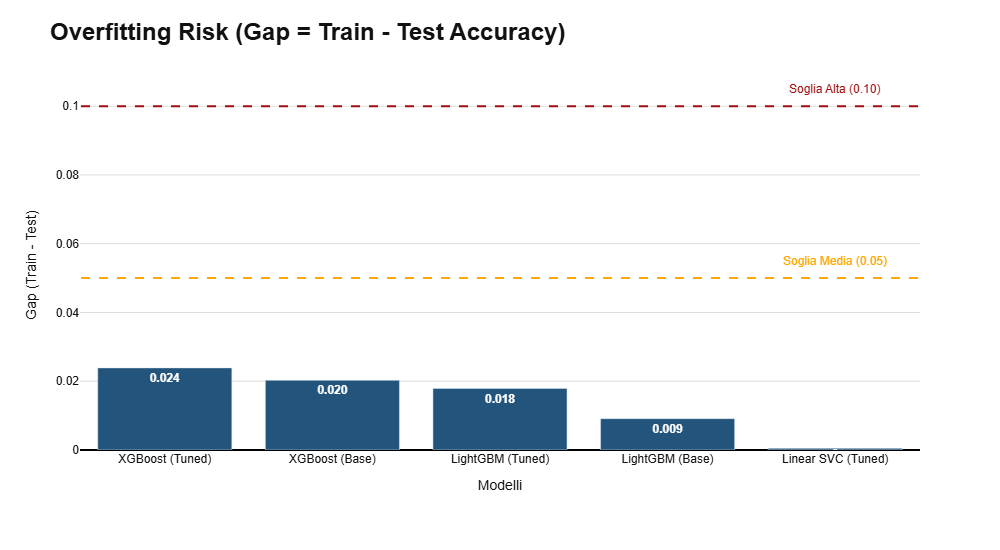
\includegraphics[width=\textwidth]{figures/overfitting.png} 
    \caption{Confronto delle accuratezze in fase di addestramento e di test. Il divario ridotto (Gap) conferma una generalizzazione stabile e un basso rischio di overfitting per tutti i modelli selezionati.}
    \label{fig:overfitting.png}
\end{figure}
